

\tikzset{every picture/.style={line width=0.75pt}} %set default line width to 0.75pt        

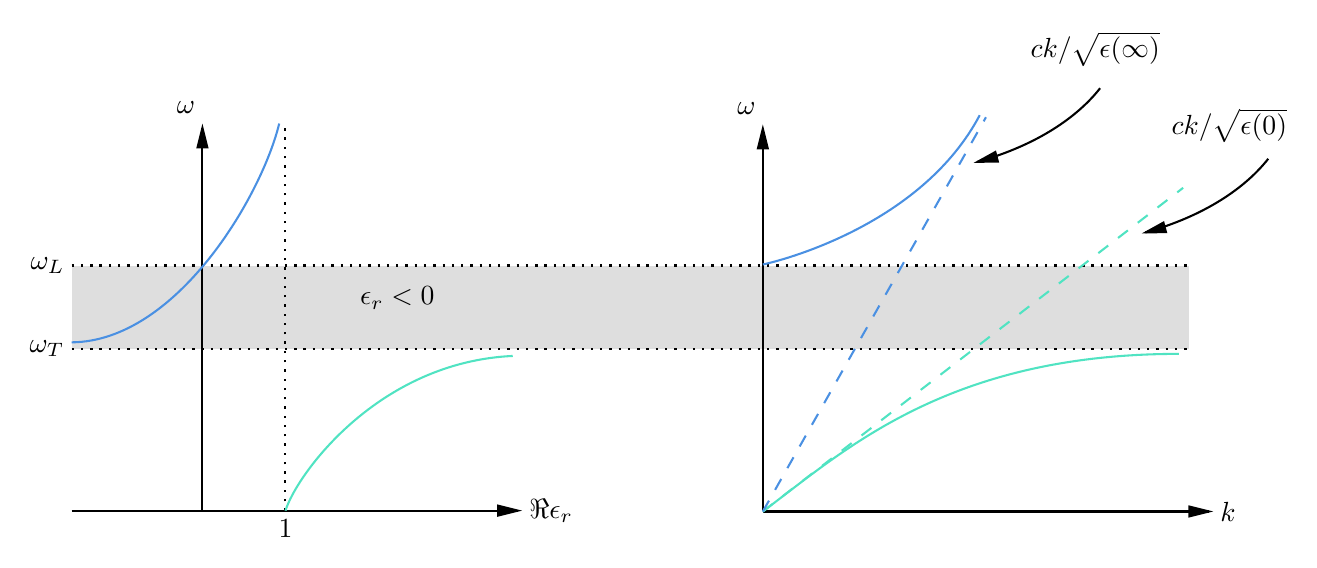
\begin{tikzpicture}[x=0.75pt,y=0.75pt,yscale=-1,xscale=1]
%uncomment if require: \path (0,335); %set diagram left start at 0, and has height of 335

%Shape: Rectangle [id:dp07379263609898756] 
\draw  [draw opacity=0][fill={rgb, 255:red, 0; green, 0; blue, 0 }  ,fill opacity=0.13 ] (45.5,157.5) -- (584,157.5) -- (584,197.5) -- (45.5,197.5) -- cycle ;
%Straight Lines [id:da1768875834879553] 
\draw [color={rgb, 255:red, 0; green, 0; blue, 0 }  ,draw opacity=1 ]   (45.5,275.58) -- (260.5,275.58) ;
\draw [shift={(262.5,275.58)}, rotate = 180] [fill={rgb, 255:red, 0; green, 0; blue, 0 }  ,fill opacity=1 ][line width=0.08]  [draw opacity=0] (12,-3) -- (0,0) -- (12,3) -- cycle    ;
%Straight Lines [id:da8310117956241199] 
\draw [color={rgb, 255:red, 0; green, 0; blue, 0 }  ,draw opacity=1 ]   (108.5,275.58) -- (108.5,91.08) ;
\draw [shift={(108.5,89.08)}, rotate = 90] [fill={rgb, 255:red, 0; green, 0; blue, 0 }  ,fill opacity=1 ][line width=0.08]  [draw opacity=0] (12,-3) -- (0,0) -- (12,3) -- cycle    ;
%Straight Lines [id:da9608764760297932] 
\draw [color={rgb, 255:red, 0; green, 0; blue, 0 }  ,draw opacity=1 ]   (378.5,276) -- (593.5,276) ;
\draw [shift={(595.5,276)}, rotate = 180] [fill={rgb, 255:red, 0; green, 0; blue, 0 }  ,fill opacity=1 ][line width=0.08]  [draw opacity=0] (12,-3) -- (0,0) -- (12,3) -- cycle    ;
%Straight Lines [id:da575210054978492] 
\draw [color={rgb, 255:red, 0; green, 0; blue, 0 }  ,draw opacity=1 ]   (378.5,276) -- (378.5,91.5) ;
\draw [shift={(378.5,89.5)}, rotate = 90] [fill={rgb, 255:red, 0; green, 0; blue, 0 }  ,fill opacity=1 ][line width=0.08]  [draw opacity=0] (12,-3) -- (0,0) -- (12,3) -- cycle    ;
%Straight Lines [id:da6187444008907346] 
\draw  [dash pattern={on 0.84pt off 2.51pt}]  (45.5,197.5) -- (584,197.5) ;
%Straight Lines [id:da06319760130839658] 
\draw  [dash pattern={on 0.84pt off 2.51pt}]  (45.5,157.5) -- (584,157.5) ;
%Straight Lines [id:da4895790172476384] 
\draw [color={rgb, 255:red, 0; green, 0; blue, 0 }  ,draw opacity=1 ] [dash pattern={on 0.84pt off 2.51pt}]  (148.5,275.58) -- (148.5,89.08) ;
%Curve Lines [id:da09047241116285987] 
\draw [color={rgb, 255:red, 80; green, 227; blue, 194 }  ,draw opacity=1 ]   (378.5,276) .. controls (418.5,246) and (468,200.06) .. (579,200.06) ;
%Straight Lines [id:da8526784873506212] 
\draw [color={rgb, 255:red, 80; green, 227; blue, 194 }  ,draw opacity=1 ] [dash pattern={on 4.5pt off 4.5pt}]  (378.5,276) -- (581,120.06) ;
%Curve Lines [id:da12354963233094818] 
\draw [color={rgb, 255:red, 80; green, 227; blue, 194 }  ,draw opacity=1 ]   (148.5,275.58) .. controls (154,258.06) and (193,204.06) .. (258,201.06) ;
%Curve Lines [id:da38900509121065796] 
\draw [color={rgb, 255:red, 74; green, 144; blue, 226 }  ,draw opacity=1 ]   (45.5,194.5) .. controls (96,194.06) and (137,124.06) .. (145.5,89.08) ;
%Curve Lines [id:da4544972239093672] 
\draw [color={rgb, 255:red, 74; green, 144; blue, 226 }  ,draw opacity=1 ]   (378.5,157) .. controls (392,154.06) and (456,136.06) .. (483,85.06) ;
%Straight Lines [id:da8551657808511666] 
\draw [color={rgb, 255:red, 74; green, 144; blue, 226 }  ,draw opacity=1 ] [dash pattern={on 4.5pt off 4.5pt}]  (378.5,276) -- (486,86.06) ;
%Curve Lines [id:da12654594371430283] 
\draw    (541,72.06) .. controls (530.22,85.78) and (510.8,99.5) .. (481.79,107.58) ;
\draw [shift={(480,108.06)}, rotate = 345.07] [fill={rgb, 255:red, 0; green, 0; blue, 0 }  ][line width=0.08]  [draw opacity=0] (12,-3) -- (0,0) -- (12,3) -- cycle    ;
%Curve Lines [id:da17190727595919086] 
\draw    (622,106.06) .. controls (611.22,119.78) and (591.8,133.5) .. (562.79,141.58) ;
\draw [shift={(561,142.06)}, rotate = 345.07] [fill={rgb, 255:red, 0; green, 0; blue, 0 }  ][line width=0.08]  [draw opacity=0] (12,-3) -- (0,0) -- (12,3) -- cycle    ;

% Text Node
\draw (264.5,275.58) node [anchor=west] [inner sep=0.75pt]    {$\Re \epsilon _{\text{r}}$};
% Text Node
\draw (597.5,276) node [anchor=west] [inner sep=0.75pt]    {$k$};
% Text Node
\draw (106.5,85.68) node [anchor=south east] [inner sep=0.75pt]    {$\omega $};
% Text Node
\draw (376.5,86.1) node [anchor=south east] [inner sep=0.75pt]    {$\omega $};
% Text Node
\draw (148.5,278.58) node [anchor=north] [inner sep=0.75pt]   [align=left] {1};
% Text Node
\draw (43.5,157.5) node [anchor=east] [inner sep=0.75pt]    {$\omega _{\text{L}}$};
% Text Node
\draw (43.5,197.5) node [anchor=east] [inner sep=0.75pt]    {$\omega _{\text{T}}$};
% Text Node
\draw (506,43.4) node [anchor=north west][inner sep=0.75pt]  [color={rgb, 255:red, 0; green, 0; blue, 0 }  ,opacity=1 ]  {$ck/\sqrt{\epsilon ( \infty )}$};
% Text Node
\draw (574,80.4) node [anchor=north west][inner sep=0.75pt]  [color={rgb, 255:red, 0; green, 0; blue, 0 }  ,opacity=1 ]  {$ck/\sqrt{\epsilon ( 0)}$};
% Text Node
\draw (183,166.4) node [anchor=north west][inner sep=0.75pt]    {$\epsilon _{\text{r}} < 0$};


\end{tikzpicture}
